\documentclass[12pt]{article}
\usepackage{myart}
% \addbibresource{/Users/lwg342/Documents/LaTeX/lib.bib}
\addbibresource{lib1.bib}
\usepackage{booktabs}\usepackage{authblk}
\usepackage{longtable}
\usepackage{tabularx}
%--------Hello World--------%
%=====================================%
\begin{document}
    \title{Augment Large Covariance Matrix Estimation With Auxiliary Network Information}
    \author[]{Shuyi Ge\thanks{Author email:sg751@cam.ac.uk}}
    \author[]{Shaoran Li\thanks{Author email:sl736@cam.ac.uk}}
    \author[]{Oliver Linton\thanks{Author email:obl20@cam.ac.uk}}
    \author[]{Weiguang Liu\thanks{Author email:wl342@cam.ac.uk}}
    \affil[]{Faculty of Economics, University of Cambridge}
    \maketitle
    % \tableofcontents
    
    \begin{abstract}
        This paper aims to incorporate auxiliary information about the location of significant correlations into the estimation of high-dimensional covariance matrices. With the development of machine learning techniques such as textual analysis, granular linkage information among firms that used to be notoriously hard to get are now becoming available to researchers. Our proposed method provides an avenue for combining those auxiliary network information with traditional economic datasets to improve the estimation of a large covariance matrix. Simulation results show that the proposed adaptive correlation thresholding method generally performs better in the estimation of covariance matrices than previous methods, especially when the true covariance matrix is sparse and the auxiliary network contains genuine information. As a preliminary application, we apply the method to the estimation of the covariance matrix of asset returns. There are several extensions and improvements that we are considering.     
    \end{abstract}
    
    \section{Model and Introduction}Our goal is to estimate \(\Sigma =\variance(y)\) where \(y\) is a \(p \times 1\) random vector, say asset returns. We collect the \(T\) observations into a matrix \(Y:p\times T\). Sample covariance estimate \(\hat{\Sigma} = \frac{1}{T} (Y - \bar{Y}\mathbf{1})(Y - \bar{Y}\mathbf{1})'\) is problematic when \(p\) is not small relative to \(T\). Popular estimation strategies include factor model, shrinkage, thresholding, banding, tapering, etc.

If in addition to the observation of \(Y\), we observe a network \(G\) among the firms, where \(G_{ij}\) either takes value \(0,1\) or a score in \([0,1]\), with higher \(G_{ij}\) implying that it's more ``likely'' that the returns of firm \(i,j\) are correlated. We show that this auxiliary network can be used to improve the estimation the covariance matrix \(\Sigma\). Examples of such network include \cite{hoberg2016TextBasedNetwork}, who identifies a product similarity network from financial reports that has been shown to be more accurate than industry block diagonal matrix. As linked firms are potentially subject to similar demand shock, we have reason to believe that \(G\) contains valuable information about the comovement among the returns.
\cite{israelsen2016does} and \cite{kaustia2020CommonAnalysts} both find that companies covered by the same analysts show similarities in many unobserved dimensions, and this analyst-based network could explain excess co-movement on top of common factors. With the development of machine learning techniques such as textual analysis, we are better at acquiring information from big data. Granular linkage information among firms that used to be notoriously hard to get due to its proprietary properties,  now are becoming available to researchers. The question is, how to use those auxiliary network information to  better estimate the co-movement between assets?

% For example, such \(G\) information could come from textual analysis, that has become more and more popular in finance, for example (\cite{fan2021HowMuch}). 

This paper aims to provide ways to extract the information contained in the auxiliary \(G\) matrix to help estimate the covariance \(\Sigma\). We consider an \textit{Adaptive Correlation Thresholding} method, where we apply thresholding to the correlation matrix, with the threshold level depending on network information. More specifically, suppose we observe \(Y_{t}\) for \(t = 1 ,\dots, T\), the procedure is 
% \begin{enumerate}
    % \item 
    % \item Guided Linear Shrinkage: we adopt the linear shrinkage method, where the shrainkge targets is chosen based on the network information. This is different from previous practice of shrinking to the identity or equicorrelation matrix. 
% \end{enumerate}

\begin{enumerate}
    \item Estimate the sample covariance estimate \(\hat{\Sigma}\), and the sample correlation matrix \(\hat{R}\). 
    \item Apply the generalized thresholding function \(h(r_{ij},\tau_{ij})\) to the off-diagonal elements of \(\hat{R} = (\hat{r}_{ij})\), as in  \cite{rothman2009GeneralizedThresholding}. The novelty is now we allow the threshold \(\tau_{ij}\) to vary across elements and to depend on the network information.  Specifications we have considered for the threshold \(\tau\) are 
    \begin{itemize}
        \item Simple linear model 
            \begin{equation*}
                \tau(G_{ij}) = a + bG_{ij}
            \end{equation*}
        \item 
        The probit model
            \begin{equation*}
            \tau_{ij} = \tau\pqty{G_{ij}} = \Phi\pqty{a + b \abs{G_{ij}}}
            \end{equation*}
    \end{itemize}
    \item Estimate the unknown parameters in the \(\tau\) function by cross validation, as in \cite{bickel2008CovarianceRegularization}, \cite{cai2011AdaptiveThresholding}, where we randomly split the sample \(V\) times, for each \(v\), compute the new estimator \(\hat{\Sigma}^{1,v}_{G}\) with the first subsample, and sample covariance \(\hat{\Sigma}^{2,v}\) and the criterion is 
    \begin{equation*}
        L(a, b) = \frac{1}{V} \sum_{v}^{V} \norm{\hat{\Sigma}^{1,v}_{G} - \hat{\Sigma}^{2,v}}^{2}_{F}
    \end{equation*}
    we find \(a,b\) that minimise this criterion. 
    
    \item Then with the estimates of \(a,b\), we can estimate \(\Sigma\) on the test sample. 
\end{enumerate}

%For the second method we consider, we construct a linear shrinkage target based on the hard-thresholded version of \(\hat{\Sigma}\), call it \(\hat{\Sigma}_{H} = [\hat{\Sigma}_{ij} \mathbf{1}\Bqty{G_{ij} > 0}]\). And apply linear shrinkage with the target. 

There are several advantages of using network guided method:
\begin{enumerate}
    \item The main advantage is that we are combining economically meaningful network with market-based performance data. Comparing to purely data-driven thresholding or shrinkage methods, the method utilizes valuable information embedded in external network data, which provides more robustness and efficiency. aif our auxiliary network contains the ``real'' links from the network. The relationship identified will be more stable over time than the relationship identified from return data alone. 
    \item This method is very flexible and extensible. Although in our current analysis we only use one of the existing networks as our proxy for $G$, you are free to include many candidate networks in the \(\tau\). You may want want to include characteristics-based distances, as it has been documented that companies with similar characteristics exhibit additional co-movement on top of common risk factors (see \cite{fernandez2011spatial} for example). It also provides a way to discern which set of information is relevant based an estimate of the coefficients \(a,b\) in the thresholding level. 
    \item The networks may provide industry-level comovement that is potentially related to the ``weak factors'' components, which we intend to investigate. 
\end{enumerate}

% There are some challanges and questions as well:
% \begin{enumerate}
    % \item Since we don't observe the true \(\Sigma\), we wonder if there are some good criteria for evaluating the performance of our \(\hat{\Sigma}\). So far I am following \cite{ledoit2004HoneyShrunk} and \cite{ledoit2017NonlinearShrinkage}. But unlike the linear and nonlinear shrinkage method, our estimator is not designed for optimal performance under the Frobenius norm. 
    % \item We don't have a quality measure of the network matrix or a model for how the \(G_{ij}\) are generated. 
    % \item In simulation studies, the optimization takes some time, but the result is not yet very robust(some times it outperforms all competitors, but sometimes the optimization will be very   off-target).
% \end{enumerate}
\section{Introduction}

Covariance matrix estimation is an important area of research in both finance and economics. Suppose we have observations $\mathbf{X}_{t}=(X_{1t},\dots,X_{Nt})^T$, $t=1,\dots,T$, that are from an $N-$dimensional random vectors with $Cov(\mathbf{X})=E(\mathbf{X}\mathbf{X}^T)={\Sigma}_{X}$. The most straightforward estimator is the sample covariance matrix, which is defined as follows:
\begin{equation}
{\hat{\Sigma}_{X}}=\frac{1}{T-1}({X}-\bar{{X}})({X}-\bar{{X}})^{\intercal}=[\sigma_{ij}]_{N\times N},
\end{equation}
where ${X}$ is the $N\times T$ matrix of observations; $\bar{{X}}=\frac{1}{T}{X}{1}_{T}{1}^{\intercal}_{T}$, with ${1}_{T}$ being a $T\times 1$ vectors of 1. However, in the high-dimensional case, where the dimension $N$ goes to infinity at a faster rate than that of the sample size $T$, the naive sample covariance matrix is ill-conditioned. Some structures need to be imposed on ${\Sigma}_{X}$, and regularisation techniques need to be applied to make sure the estimator is reliable. In particular, we usually assume that ${\Sigma}_{X}$ is sparse (i.e., has lots of zeros) or conditionally sparse (i.e., has lots of zeros once we condition on some variables like the common risk factors).

To proceed under sparsity, the key job is to find out the location of non-zero entries. There are two broad categories of regularisation, namely banding and shrinkage.  Banding is applicable when $X_{it}$ is indexed, and we can expect that larger $|i-j|$ implies lower correlation. Such structure is appropriate for applications where there are natural orderings of variables, such as climatology and spectroscopy. \cite{bickel2008regularized} regularize the ${\hat{\Sigma}_{X}}$ in a way that, for a typical entity $i$, only the set of neighours defined by $\{j\in {N_i}: |i-j|\leq \rho, j=1,\dots,N \}$ have non-zero covariances with $i$. Other $j$s with $|i-j|>k$ have $\sigma_{ij}=0$. When $X_{it}$ is not indexed, we may apply some shrinkage techniques to the off-diagonal elements of ${\hat{\Sigma}_{X}}$, and achieve sparsity by setting relatively unimportant entries that are smaller than a data-driven threshold to zeros.  In general, we have ${\tilde{\Sigma}_{X}}=[\tilde{\sigma}_{ij}]_{N\times N}$, where
\begin{equation}
    \tilde{\sigma}_{ij}=\left\{ \begin{array}{cc}
      \hat{\sigma}_{ii}   & i=j \\
       s_{\lambda}(\hat{\sigma}_{ij})  & i\neq j
    \end{array}\right.,
\end{equation}
where $s_{\lambda}(\cdot)$ is a shrinkage function with $\lambda$ being a tuning parameter, satisfying (1) $|s_{\lambda}(\mu)|\leq|\mu|$ for $\mu \in \mathcal{R}$; (2) $s_{\lambda}(\mu)$ if $|u|\leq \lambda$; (3) $|s_{\lambda}(\mu)-\mu|\leq \lambda$. \citet{bickel2008covariance} develop a universal threshold for all entries. \citet{cai2011adaptive} establish entry-adaptive threshold to ${\hat{\Sigma}_{X}}$. \citet{fan2013large} argue that common factors should be extract first before applying thresholding selection when there are "extremely spiked" eigenvalues in ${\hat{\Sigma}_{X}}$ (i.e., the covariance matrix is conditionally sparse). 

Another way of shrinkage is via penalization. \citet{yuan2007model}, \citet{d2008first}, \citet{rothman2008sparse} and \citet{friedman2008sparse} among others employ LASSO type penalty to shrink sample covariance matrix. Another seminal penalty choice is SCAD, which is proposed by \citet{fan2001variable}, can be found in \citet{fan2009network} and \citet{lam2009sparsistency}.

However, most of these shrinkage approaches rely on ${X}$ only and ignore information about pairwise relationships beyond the observed data ${X}$, which may suffer a loss especially in a information-abundant era. When $X_{it}$ is not indexed, we are not be able to have strong implications in terms of the locations of non-zeros as in \cite{bickel2008regularized}. However, we do have some idea that who might be connected with whom using augment information apart from ${X}$. To proxy for pairwise connectivity among entities, apart from purely statistical methods, there have been other ways. \citet{hoberg2016text} use textual analysis to identify peers. \cite{kaustia2013common} identify peers analyst co-coverage, and \cite{ge2021news} identify peers using business news co-mentioning. Those network information gathered from other sources can help us to identify the locations of non-zeros apart from the information from ${X}$ itself. Similar location-based thresholding ideas have applied in \cite{fan2016incorporating} and \citet{brownlees2020community}. \cite{fan2016incorporating} apply a hard thresholding method in a way that $\sigma_{ij}=0$ when $i$ and $j$ are from different sector/industry. \citet{brownlees2020community} first detect community structure using a spectral clustering-based procedure, and then apply a block-by-block thresholding to the off-diagonal elements of ${\hat{\Sigma}_{X}}$. In particular, they do not apply and thresholding to $\hat{\sigma}_{ij}$ if $i$ and $j$ are from the same community.

In this paper, we utilize granular network information gathered from other sources that could imply the locations of non-zeros in the de-factored residuals covariance matrix. The first candidate is the new-implied network. It has been documented that common news coverage reveals information about linkages among companies, which are related to many economically important relationships like business alliances, partnerships, banking and financing, customer-supplier, and production similarity (\citet{scherbina2015economic}, \citet{schwenkler2019network}). \cite{ge2021news} document that stocks linked by news co-mentioning exhibit additional co-movement beyond what can be explained by common risk factors. Same as \cite{ge2021news}, we use news data from RavenPack Equity files Dow Jones Edition for the period between the beginning of 2004 to the end of 2015. This comprehensive news dataset combines relevant content from multiple sources, including Dow Jones Newswires, Wall Street Journal, and Barron’s  MarketWatch, which produce the most actively monitored streams of news articles in the financial system. We identify linkages among firms by news co-mentioning. The second candidate network is IBES analyst co-coverage network. \cite{israelsen2016does} documents that stocks linked by analysts exhibit excess comovement. To construct the analyst co-coverage-based adjacency matrix, we use the Institutional Brokers Estimate System (IBES) detail history files. (after getting the network, our procedure)?


Although here we are applying augment network information to the estimation of large static covariance matrix, similar idea can be extended to the estimation of large dynamic covariance matrix. For example, dynamic network information could be well incorporated into the conditioning information set in \citet{chen2019new}.


\section{Data}
We consider daily returns of $S\& P$ $500$ stocks for our application. All the stock market related data are from the Center for Research in Security Prices (CRSP). Daily factor returns are obtained from Kenneth French’s website.
\subsection{News Implied Network}
The news data are obtained from RavenPack Equity files Dow Jones Edition for the period January 2004 to December 2015. This comprehensive news dataset combines relevant content from multiple sources, including Dow Jones Newswires, Wall Street Journal, and Barron's MarketWatch, which produce the most actively monitored streams of news articles in the financial system. Each unique news story (identified by a unique story ID) tags the companies mentioned in the news by their unique and permanent entity identifier codes (RP\_ENTITY\_ID),  by which we link to stock identifier TICKER and PERMNO.

As as \cite{ge2021news}, we identify links by news co-mentioning. That is, if a piece of business news reports two companies together, they share a link. We do not consider news that co-mention more than two companies since although news they may carry potential information about links, they provide noisier information. We also remove news with topics including analyst recommendations, rating changes, and index movements as these types of news might stack multiple companies together when they actually do not have real links. \autoref{table:news} provides descriptive statistics for RavenPack Equity files Dow Jones Edition dataset during the sample period. Since our comprehensive news dataset combines several sources, given a similar length of sample period, the number of unique news stories is more than ten times larger than that from \citet{scherbina2015economic} and more than eight hundred times than that from \citet{schwenkler2019network}. For link identification purposes, we only use sample news (1) are not about topics mentioned above (2) tag $S\& P$ $500$ companies and (3) mention exactly two companies, which is a subsample of $1,637,256$ unique news stories.

\subsection{IBES Analyst Coverage Network}
We use the Institutional Brokers Estimate System (IBES) detail history files to construct the analyst co-coverage-based adjacency matrix. For each year in the sample, we consider a stock is covered by an analyst if the analyst issues at least one FY1 or FY2 earnings forecast for the stock during the year. And we consider two stocks as linked if there are common analysts during the year, weighted by the number of common analysts. 

    \section{Literature Review}    % With the technology such as machine learning based textual analysis, we have acquired a lot of auxiliary information about the linkage between companies, industries and so on. Can we use that information to better estimate the co-movement between assets?
    There has been extensive research on high-dimensional covariance estimation. Some important lines of thinking include element-wise banding and thresholding method, shrinkage method, factor models, etc. For a book-length review see \cite{pourahmadi2013HighdimensionalCovariance}.\\
    
    \cite{bickel2008CovarianceRegularization} considers banding or tapering the sample covariance matrix. \cite{bickel2008CovarianceRegularization} considers covariance regularization by hard thresholding. They also compare the results between banding when there is a natural ordering(for example, time series autocorrelation) and thresholding where we need to pay a \(\log p\)  price in the convergence rate to learn the locations. 
    \cite{cai2011AdaptiveThresholding} considers adptive thresholding where threshold takes the form:
    \begin{equation}
        \hat{\sigma}_{ij}^{*} = s_{t_{ij}}\pqty{\hat{\sigma}_{ij}}
    \end{equation}
    where \begin{enumerate*}
        \item \(\abs{s_{\lambda}(z)} \leq c \abs{y}\) for all \(\abs{z - y}\leq \lambda\)
        \item \(s_{\lambda}(z) = 0\) for \(\abs{z}\leq \lambda\)
        \item \(\abs{s_{\lambda}(z) - z} \leq \lambda\).
    \end{enumerate*}
    The convergence rate is the same, although here the uniformity class is larger. \cite{fan2015OverviewEstimation} proposes thresholding on the correlation matrix. The choice of thresholding functions can be found \cite{rothman2009GeneralizedThresholding}, \cite{fan2001VariableSelection}, etc. \\
    
    As an application of thresholding method, \cite{fan2016IncorporatingGlobal} use hard thresholding method in a high-frequency setting based on the sector/industry classifier. \(s_{ij}(\sigma_{ij})= \sigma_{ij}\) if \(ij\) are in the same industry. The network they use is a block-diagonal matrix and our results accommodate more general and flexible network information. \\

    \cite{ledoit2004HoneyShrunk} develops an estimation strategy based on linear shrinkage, where the target is identity matrix. This shrinkage guarantees that the estimated covariance matrix is well-conditioned. This approach can be thought of as decreasing variance at the expense of increasing bias a little. There are articles discuss multiple targets, for example, \cite{schafer2005ShrinkageApproach}, \cite{lancewicki2014MultiTargetShrinkage} and \cite{gray2018ShrinkageEstimation}, but their targets are either fixed or data-driven, so different from our guided method where we bring in new information from auxiliary network information. 
    \cite{ledoit2012NonlinearShrinkage} and \cite{ledoit2017NonlinearShrinkage} propose nonlinear shrinkage where the eigenvalues are pulled towards the ``correct level'' solving a nonrandom limit loss function. The shrinkage method has been shown to have really good performance in estimating large-dimensional covariance matrix, however they are a global method whereas our method is designed to emphasize ``economically meaning'' links. There is also a vast literature on factor models in high-dimensional models and applications in empirical finance. We refer to \cite{connor2012EfficientSemiparametric}, \cite{fan2015OverviewEstimation} and \cite{fan2016ProjectedPrincipal} and literature review therein. 
    \section{Simulations}We demonstrate the Network Guided Estimator and examine its small-sample performance using the following simulations. First, we consider the case where the true covariance \(\Sigma\) comes from an AR(1) model. So for \(\Bqty{(i,j): i =1 ,\dots, N, j = 1,\dots,N} \), \(\sigma_{ij}^{2} = \sigma_{i}\sigma_{j} \rho_{ij}\) and \(\rho_{ij} = \rho^{\abs{i - j}}\), we take \(N = 200\) and  
\begin{equation*}
     \sigma_{ij} = 3 * \rho^{\abs{i - j}}. 
\end{equation*}
Assume we observe a matrix \(\hat{L}\) indicating the location of highly correlated pairs \(L_{ij} = \mathbf{1}\Bqty{\rho_{ij} \geq l}\). Conditional on \(L_{ij} = 1\), we observe \(\hat{L}_{ij}= 1\) with probability \(p\) and conditional on \(L_{ij}  =0\) , \(\hat{L}_{ij}  =1\) with probability \(q\). Hence \(p,q\) reflect the probability of missing important locations (type \RN{2} error) and including falsely important locations (type \RN{1} error) respectively. 

We then generate \(T = 100\) independent draws of observations \(X_{t}\) from \(N(0, \Sigma)\) and estimate \(\Sigma\) using 
\begin{enumerate*}
     \item Sample covariance;
     \item Linear Shrinkage estimator;
     \item Nonlinear Shrinkage estimator;
     \item Universal thresholding on the correlation;
     \item and Network Guided Estimator. 
\end{enumerate*}
We now compare their performance. It's worth collecting here the parameters that we will adjust in the experiments in \autoref{t:1}
\begin{table}[htbp]
     \centering\begin{tabularx}{\textwidth}{c|X}
          \toprule
          Parameter & Description \\ 
          \midrule
          \(\rho\) & Determines how strong the correlation is and the sparsity of the covariance matrix \(\Sigma\) \\
          \(l\) & Observation level, determines how we classify a pair \((i,j)\) as important, i.e., \(L_{ij} =\mathbf{1}\Bqty{\rho_{ij} > l}\). \\
          \(p\) & Conditional on \(L_{ij} =1\), the probability of actually observing \(\hat{L}_{ij} =1\). \\
          \(q\) & Conditional on \(L_{ij} = 0\), the probability of  observing \(\hat{L}_{ij} =1\)\\
          \(\lambda\)& The Threshold level when we apply generalized thresholding operator on \(\sigma_{ij}\) where \(\hat{L}_{ij} = 0\). \\
          \bottomrule
     \end{tabularx}
     \caption{Description of varying parameters.}
     \label{t:1}
\end{table}


In Table \ref{t:2-2}, \ref{t:2-fro} and \ref{t:2-1}, we show the estimation errors of these estimators in terms of the operator norm, the Frobenius norm and the matrix 1-norm, when we simulate using different \(\rho\) and thresholding level \(\lambda\) and fix the other parameters at \(l = 0.3, p = 1\) and \(q =0\). Here we have taken the thresholding operator to be soft thresholding. It can be seen that for all these norms, when the true covariance matrix is not too dense, Network Guided Estimator outperforms all the competitors given a good choice of $\lambda$. When the true covariance matrix is more sparse, indicated by smaller $\rho$, thresholding methods become more appealing and when the true covariance matrix is denser, the sample covariance estiamtor shows better performance compared with other benchmark models. Thanks to the accurate location information, Network Guided Estimator is able to balance these two estimators.  

% When the covariance matrix becomes denser, the advantages of Universal Threshold are vanishing, even under well-chosen Threshold level $\lambda$. However, with the assistance of the network guidance, the excellent performance is preserved, except for the extreme circumstance where $\rho=0.99$.

Another tuning parameter in the Network Guided Estimator is the choice of $l$, which can determine whether a link should be reserved regardless of the information from the statistic. Then we consider simulations with varying observation levels \(l\). In Figure \ref{fig:1}, \ref{fig:2}, \ref{fig:3}, 
when we set observation level equal to \(0\), the Network Guided Estimator will be the same as the sample covariance estimator, on the other extreme, when observation level is set to \(1\), the Network Guided Estimator is equivalent to universal thresholding. In between these cases, when we have information about the locations of the important pairs, we have a range where the estimation errors can be lowered. 

Then we show the effects of errors in estimating the \(L_{ij}\) by varying the parameters \(p\) and \(q\). In Table \ref{t:3-2}, \ref{t:3-fro}, \ref{t:3-1}, we have when \(p = q = 0\) the estimation error of the universal thresholding estimator, and \(p =q =1\) the sample covaraince estimation error. As we can see, as long as \(q\) is not too large, the estimation error will be smaller when we have a higher probability \(p\) of observing the true large elements. It should be noted that \(q\) in fact cannot be very large, given that the whole matrix is sparse.  
    \section{Empirical Studies}In this section, we apply the adaptive correlation thresholding method to a portfolio construction problem. First we describe the procedure and then present some of the results we have. 

Assume we observe the excess return \(Y_{it}\), \(i = 1,\dots,N\) and \(t= 1,\dots, T\) follows
\begin{equation*}
    Y_{it} = B_{i}' F_{t} + u_{it} ; \quad \Sigma_{u} = E(u_{t}u_{t}')
\end{equation*}
where \(F_{t}\) are factor excess returns. Here we have considered Fama-French 3 and the Carhart's momentum factor. The goal is to estimate \(\Sigma_{Y} = E\pqty{YY'}\) and use that estimate to construct portfolio following \cite{ledoit2017NonlinearShrinkage}. The auxialiary network we have include the \cite{hoberg2016TextBasedNetwork}'s network(henceforth Hoberg's Network) and IBES analysts cocoverage network. Here we present the results for SP500 returns using Hoberg's Network. 

The procedure we take is as follows. 
\begin{enumerate}
    \item We run time series linear regressions of \(Y_{it}\) on \(F_{k,t}\), obtain the beta estimates \(\hat{B}_{i}\) and the residual \(\hat{u}_{it}\). 
    \item Compute the covaraince matrix \(S_{\hat{u}} = \frac{1}{T}\hat{u}\hat{u}'\) and \(S_{F} = \frac{1}{T} \sum_{t} (F_{t} - \bar{F})(F_{t} - \bar{F})'\) and appply \textit{adaptive correlation thresholding} on \(S_{\hat{u}}\), denote the estimate as \(\hat{S}_{\hat{u}}\). 
where the second step adaptive correlation thresholding is achieved in the following way. Let \(R_{u}\) be the correlation matrix calculated from \(S_{u}\). We use soft thresholding \(h(r_{ij}, \tau_{ij}) = \sign\pqty{r_{ij}} \pqty{r_{ij} - \tau_{ij}}_{+}\) on the off-diagonal elemetns \(r_{ij}\) of \(R_{u}\), where 
\begin{equation*}
    \tau_{ij} = \delta_{ij} \sqrt{\frac{\log N}{T}}
\end{equation*}
and 
\begin{equation*}
    \delta_{ij} = a + b G_{ij}
\end{equation*}

% \blue{(so that the network is a little denser, and I have also considered specification of \(\delta\) as a probit model, but it complicates the optimization part because the constraint is nonlinear.)}. 

Let the threshold estimate be \(\hat{R}_{\hat{u}}(a,b)\), given \(a,b\), our estimate will be
\begin{equation*}
    \hat{S}_{\hat{u}} = \hat{S}_{\hat{u}}(a,b) = \diag(S_{\hat{u}})^{\frac{1}{2}} \hat{R}_{\hat{u}}\diag(S_{\hat{u}})^{\frac{1}{2}}
\end{equation*}

In order to guarantee positive definiteness, I follow the suggestion in \cite{fan2015OverviewEstimation} and \cite{fan2013LargeCovariance}, by first finding the minimum \(\underline{\delta}\) such that the \(\hat{S}(\delta, 0)\) has its smallest eigenvalue larger than \(0\) if we choose \(\tau_{ij} = \underline{\delta} \sqrt{\frac{\log N}{T}}\). 

Then \(a,b\) are estimated using cross-validation following \cite{bickel2008CovarianceRegularization} by randomly spliting the sample \(V\) times, for each \(v = 1,\dots,V\), compute the estimate \(\hat{S}^{1,v}_{u}\) with the first subsample, and sample covariance estimate \(\hat{\Sigma}^{2,v}_{u}\) with the second subsample and let the criterion function be
\begin{equation*}
    L(a, b) = \frac{1}{V} \sum_{v}^{V} \norm{\hat{S}^{1,v}_{u} - \hat{\Sigma}^{2,v}_{u}}^{2}_{F}
\end{equation*}
we find \(\hat{a},\hat{b}\) that minimise this criterion subject to the constraints:
\begin{align}
    0 \leq a \sqrt{\frac{\log N}{T}} &\leq 1 \\
    b \sqrt{\frac{\log N}{T}} &\leq 0 \\
    \underline{\delta} &\leq a + b 
\end{align}
\item Construct an estimate of \(\Sigma_{Y}\) by \(\hat{\Sigma}_{Y} = \hat{B}S_{F}\hat{B}' +\hat{S}_{\hat{u}}\)
\end{enumerate}

We have estimated the covariance matrices of SP500 stocks from 1996 to the end of 2017; using stock return data and Fama-French 3 factor returns \(F_{kt}, k =1,2,3\). We incorporate Hoberg's network \(G_{t}\) that are updated yearly into our estimation procedure. 

The Hoberg's Network is a yearly updated \(N\times N\) network with elements in \([0,1]\) with higher score \(G_{ij}\) reflecting potentially higher correlation between the \(i\)-th and \(j\)-th firms.


In Figure 1, we present the distribution, we present the distribution (blue) of sample covariance estimates \(S_{\hat{u}, ij}\) of residuals after regressing the the stocks returns on the Fama-French 3 factor for the stocks that haIn Figure 1, we present the distribution (blue) of sample covariance estimates \(S_{\hat{u}, ij}\) of residuals after regressing the the stocks returns on the Fama-French 3 factor for the stocks tsiduals after regressing the the stocks returns on the Fama-French 3 factor for the stocks that have no missing data in the dataset; alongwith the distribution of  sample covariance \(S_{\hat{u},ij}\) for those \(ij\) with \(G_{ij} > 0\) in the Hoberg's network. It's clear that the distribution is shifted to the right, implying that Hoberg's network can pick up information that are not explained by the factors. 

\begin{figure}[htbp]
    \centering
    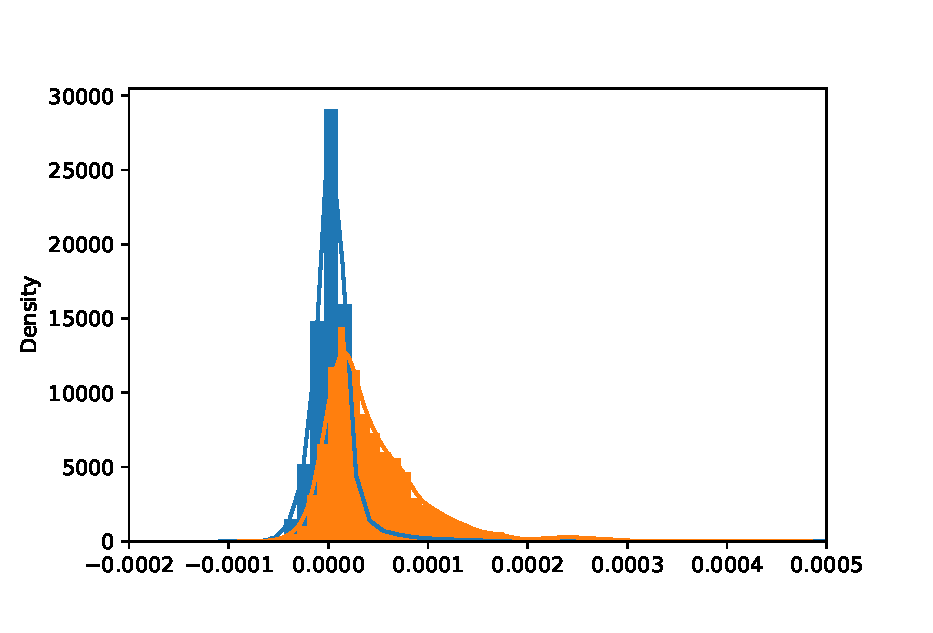
\includegraphics{fig1.eps}
    \caption{Distribution of \(S_{\hat{u},ij}, i,j = 1,\dots,N\) and \(S_{\hat{u},ij}\) for \(i,j\) such that \(G_{ij} >0\) }
    \label{<label>}
\end{figure}

Then we use a rolling-window estimation, with 252-day estimation period and then move the window forward by 21 days. In the estimation periods in window  \(m= 1, \dots,M\) we construct estimate \(\hat{\Sigma}_{Y,m} = \hat{B}S_{F}\hat{B}' + \hat{S}_{\hat{u}}\pqty{\hat{a}_{m}, \hat{b}_{m}}\). The estimated parameters \(\hat{a}_{m},\hat{b}_{m} \)  have mean \((1.177, -0.252)\), where the \(\hat{b}\) measures the effect of knowing the auxiliary network on the thresholding level. 

    \section{Conclusion and Further Works}This paper considers the problem of incorporating ever-increasing auxialiary data from machine learning techniques such as textual analysis into the estimation of large covariance matrices. 
This current version is preliminary with ongoing research on the following  applications.

Firstly, we are applying the covaraince estimation technique on portfolio construction, following the problem considered in \cite{ledoit2004HoneyShrunk} and \cite{ledoit2017NonlinearShrinkage}, where the estimation of the sparse covaraince matrices are vital for constructing the minimum-variance portfolio. 

Secondly, the method can be applied to study spatial-APT under large \(N\) case. \cite{kou2018asset} finds that common risk factors are insufficient to capture all the significant inter-dependencies in asset returns, and local interactions are also important.  Spatial-APT and spatial CAPM type of models have not been popular in large N case since the measure of contiguity is challenging. Our method can uncover contemporaneously correlated entities by combining market-based information and auxiliary network information, thus providing a natural contiguity measure. Relying solely on either statistical methods or external network information is not as desirable as the links identified by the former are hard to interpret and the external network may miss some important links.

Thirdly, we are expanding the set of auxialiary networks beyond the Hoberg's network as well as applying the technique on larger datasets. We have collected IBES analysts cocovarage network and are constructing new network based on firms' characteristics. The flexibility of the methods allows us many potential improvements. 

    % \section{Log}% \subsection{2020-08-21}
Can we build a full probability model for such problem. Suppose that \(y: {\Omega}\to \mathbb{R}^{p}\) be a random vector that has finite second moment. 
\begin{equation}
    \Sigma = \variance(y) = \bqty{\sigma_{ij}}_{i,j = 1,\dots,p}
\end{equation}

Suppose there is an observation matrix \(G_{t} = \bqty{g_{ij}}_{ij, t}\) for each time \(t\). 
\begin{equation}
    g_{ij,t} = \Phi\pqty{\theta_{1} \rho_{ij} + f(z_{i},z_{j})}
\end{equation}
where \(\rho_{ij}\) is the correlation coefficient. 
We can estimate \(\theta_{1}\) and \(f\) is a symmetric function, it could be \(\theta_{2} (z_{i} + z_{j})\), and \(z\) are asset characteristics such as size: larger firms have more media exposure. 

How to combine the two sets of information. Assume a DCC dynamic:
\begin{equation}
    \Sigma_{t} = D_{t}^{\frac{1}{2}} R_{t} D_{t}^{\frac{1}{2}}
\end{equation}
where \(D_{t}\) individually follows GARCH(1,1), \(R_{t}\). 

In DCC, \(R_{t}\) is written as \(r_{ij,t} = \frac{q_{ij,t}}{\sqrt{q_{ii,t} q_{jj,t}}}\) where \(q_{ij,t}\) follows GARCH, or exponential smoothing. 
\begin{equation}
    q_{ij,t} = \bar{\rho}_{ij,t} + \alpha \pqty{\epsilon_{i,t-1} \epsilon_{j,t-1} - \bar{\rho}_{ij}} + \beta \pqty{q_{ij,t} - \bar{\rho}_{ij}} 
\end{equation}

\subsection{2020-08-22}
I have tried to simulate covariance matrix, see simulation codes. Notice that in Bickel and Levina, they showed that banding is more efficient when the index has meaning.

Really it's about the model for \(g_{ij} = \mathbf{1}\pqty{\rho_{ij} > \tau}\). 
\begin{equation}
    P(g_{ij} = 1) = \Phi\pqty{\theta_{1}\rho_{ij} + \theta_{2} z_{1} + \theta_{3}z_{2}}
\end{equation}

Then we choose that \(\tilde{\rho}_{ij}\) that are significantly nonzero. 


\subsection{2020-09-01}
Based on the projection idea, suppose we have several estimator \(S_{1},\dots,S_k\) that besides the sample covariance matrix \(S_{0}\), we want to project \(\Sigma: n\times n\) from observations over \(t =1 ,\dots,T\) on \(I, S, S_{1},\dots S_{k}\). Suppose \(k = 1\), then we want to find the projection with the inner product defined on the space of random matrices :
\begin{equation}
    \ip{A}{B} = E \frac{1}{n} \tr[AB^{\top}]
\end{equation}

Then we have \(\Sigma = aI + \beta_{0}S_{0} + \beta_{1}S_{1}\), the oracle coefficients are 
\begin{equation}
    \bmqty{a \\ \beta_{0} \\\beta_{1}} = \bmqty{\norm{I}^{2} & \ip{S_{0}}{I} & \ip{S_{1}}{I} \\ \ip{I}{S_{0}} & \norm{S_{0}}^{2} & \ip{S_{1}}{S_{0}} \\ \ip{I}{S_{1}} & \ip{S_{0}}{S_{1}} & \norm{S_{1}}^{2} }^{-1}
    \bmqty{ \ip{\Sigma}{I} \\ \ip{\Sigma}{S_{0}}\\ \ip{\Sigma}{S_{1}}}
\end{equation}

Each quantity can be estimated by the sample counterpart, i.e. replacing \(\Sigma\)  with \(S_{0}\). We do a simulation.

But this is wrong, because we almost always fully load on the sample covariance matrix. I think it's because we can't simply replace the quantities with sample counterparts.

Suppose we have two estimators \(S_{1}, S_{2}\) for \(\Sigma\), we want to find \(\Sigma^{*} = \alpha I +\sum_{j}\beta_{j}S_{j}\) such that \(E \norm{\Sigma^{*} - \Sigma}^{2}\) is minimised. 

\begin{align}
    E \norm{\Sigma^{*} - \Sigma}^{2} = E\ip{ \alpha I +\sum_{j}\beta_{j}S_{j} - \Sigma}{\alpha I +\sum_{j}\beta_{j}S_{j} - \Sigma} 
\end{align}

Define 
\begin{align}
    \mu := \ip{\Sigma}{I} = E \ip{S_{1}}{I} =: \mu_{1}\\
    \mu_{2} := E \ip{S_{2}}{I} = E\bqty{\frac{1}{n} \tr S_{2,n}}
\end{align}

\red{Need to think about what can and cannot be directly estimated}
\subsection{2020-09-03}

We have on the LHS: 
\begin{equation}
    \bmqty{\ip{\Sigma}{I} \\\ip{\Sigma}{S_{1}} \\ \ip{\Sigma}{S_{2}}}
\end{equation} 
which involves unknown quantity \(\Sigma\).

\begin{align}
    \ip{\Sigma}{I}& = E \ip{S}{I} = E \frac{1}{n} \tr(S) \\
    &= \frac{1}{n} E \tr(\frac{1}{T} \sum x_{t}x_{t}')
\end{align}
which can be estimated with 
\begin{equation}
    \frac{1}{n} \frac{1}{T} \tr \pqty{\sum_{t} x_{t} x_{t}'}
\end{equation}

\subsection{2020-09-04}
The linear shrinkage is just projection with the inner product defined by \(\ip{A}{B}_{E} = E \ip{A}{B}\) for \(A, B\) random matrices taking value in the space of psd real matrices. 

\subsection{2020-10-10}:
Now lets consider if we can estimate the inner product between \(\Sigma\) and a another matrix \(A\), for which we have repeated observations such as the sample covariance \(S\). 

Let there be \(y_{t}: t = 1,\dots,T\), then we have 
\begin{equation*}
    S_{t} = y_{t} y_{t}' \qq{and} S = \frac{1}{T} \sum^{T} S_{t}f
\end{equation*}

The inner product is defined on random matrices: 
\begin{defn}
    Let \(A, B\) be random \(n\times n\) matrices, define 
    \begin{equation*}
        \ip{A}{B} = E \frac{1}{n} \tr(AB')
    \end{equation*}
\end{defn}

Then we can estimate \(\ip{\Sigma}{I} = E \frac{1}{n} \tr\pqty{\Sigma}\) by
\begin{equation*}
    \frac{1}{T} \sum_{t} \frac{1}{n}\tr\pqty{S_{t}}
\end{equation*}

For \(\ip{\Sigma}{S} = E \frac{1}{n} \tr\pqty{\Sigma S'}\), 
\begin{align*}
    \ip{\Sigma}{S} &= E \frac{1}{n} \sum_{i}\sum_{j} \sigma_{ij}s_{ij} \\
    &=  \frac{1}{n} \sum_{i}\sum_{j} \sigma_{ij}^{2}\\
    &= \ip{\Sigma}{\Sigma}
\end{align*}

\(\ip{\Sigma - S} = \norm{\Sigma}^{2} - \ip{S}{\Sigma} - \ip{\Sigma}{S} + \norm{S}^{2} = \norm{S}^{2} - \ip{\Sigma}{S}\). 

For the part
\begin{align}
    \norm{S}^{2} &= E \frac{1}{n} \sum_{i} \sum_{j} s_{ij}^{2} \\
    &= \frac{1}{n} E \sum_{i}\sum_{j} \pqty{\pqty{s_{ij} - \sigma_{ij}}^{2} + \sigma_{ij}^{2} } \\
    &= \frac{1}{n} \sum_{i}\sum_{j}E \pqty{\frac{1}{T} \pqty{\sum_{t} y_{it}y_{jt}'} - \sigma_{ij}}^{2} + R
\end{align}
the first term is just the variance of \(s_{ij}\) which is an estimate of \(\sigma_{ij} =  \covariance(y_{i}, y_{j})\). We can estimate it with:
\begin{equation*}
    \frac{1}{T} \pqty{\sum_{t} s_{t,ij} - s_{ij}}^{2}
\end{equation*}

Then consider a general \(A\):
\begin{align*}
    \ip{\Sigma}{A} &= \frac{1}{n} \sum_{i}\sum_{j} \sigma_{ij}a_{ij} \\
    &= \frac{1}{n} \sum_{i}\sum_{j} \sigma_{ij} E\pqty{a_{ij}}
\end{align*}

What's important is when \(a_{ij}\) and \(s_{ij}\) are not independent and when \(a_{ij}\) are not unbiased.
\subsection{2020-10-16}
Imagine the eigendecompositon, we are finding rank \(k\) approximation of \(\Sigma\). With the information in \(G\), suppose we have 
\begin{equation*}
    \norm{\Sigma - \Sigma \mathbf{1}_{G}} \qq{is small.}
\end{equation*}

Then \(G\) contains information that's useful.
\subsection{2020-11-09}
There are several questions:
\begin{enumerate}
    \item Does the network informs about the comovement?
    \item Now I think the best way is to combine the factor model, the shrinkage method and the network information. 
\end{enumerate}

\subsection{2020-11-12}

A network of cointegration relationship. 

\subsection{2020-11-18}
    Suppose we have a sparsity matrix to estimate, if we have some information about which location has zero elements: \(\sigma_{ij} = 0\), suppose this information is independent across \(ij\). Our estimate \(S^{*} = [S^{*}_{ij}]\) will try to minimise the Frobenius Norm: 
    \begin{equation*}
        \min E \sum_{i}\sum_{j} \pqty{\sigma_{ij} - s^{*}_{ij}}^{2}
    \end{equation*}
    
    Suppose we know the probability of \(\sigma_{ij} \neq 0\): \(p_{ij} = p(G_{ij}, X_{i}, X_{j})\) exactly, then suppose our sample estimation is \(s_{ij}\), for each element the expectation of MSE is:
    \begin{equation*}
        p_{ij} E (s_{ij} - \sigma_{ij})^{2} + (1-p_{ij}) E \pqty{s_{ij}^{2}} = E\pqty{s_{ij} - \sigma_{ij}}^{2}
    \end{equation*}
    if we use \(s_{ij}\) to estimate \(\sigma_{ij}\), the MSE of using \(0\) as estimate is:
    \begin{equation*}
        p_{ij} \sigma^{2}_{ij} 
    \end{equation*}
    so we would include \(s_{ij}\) if \(p_{ij}> \frac{E\pqty{s_{ij} - \sigma_{ij}}^{2}}{\sigma^{2}_{ij}}\)
    
    \subsection{2020-11-18}
    I have moved the original introduction section here. 
    \begin{question}
        Can we incorporate the information from \(G\) in the estimation of \(\Sigma\). I have thought of several ways:
    \end{question}

    \begin{enumerate}
        \item \textbf{Hard thresholding}: suppose we estimate the elements \(\sigma_{ij}\) in  \(\Sigma\) with \(s_{ij,G}(\hat{\sigma}_{ij})\), where \(\hat{\sigma}_{ij}\) are the sample covariance estimates, and \(s_{ij,G}\) is a hard-thresholding operator:
        \begin{equation}
            s_{ij,G}(\hat{\sigma}_{ij})
            \begin{cases}
                \hat{\sigma}_{ij} \qq{if} G_{ij} =1 \qq{or} i=j \\
                0 \qq{otherwise}
            \end{cases}
        \end{equation}

        Let the estimated matrix be \(\hat{S}_{G} = \pqty{s_{ij,G}(\hat{\sigma}_{ij})}_{i,j = 1,\dots, N}\). 
        \cite{bickel2008RegularizedEstimation} compares the difference between thresholding and banding and finds intuitively that if the assets are ordered in a meaningful way, then banding is more efficient than thresholding. Our method is like banding with ``order'' implied by \(G\). 

        \cite{fan2016IncorporatingGlobal} considers the hard thresholding where they only keep the \(\hat{\sigma}_{ij} \) for which \(i,j\) are in the same industry, so their \(G\) is just a block diagonal matrix. I think it will miss some important links. 

        \item \textbf{Shrinkage}: \cite{ledoit2004WellconditionedEstimator} considers finding a linear combination of sample covariance matrix \(\hat{\Sigma}\) and the shrinkage target \(I\) that minimizes the mean squared estimation error in Frobenius norm:
        \begin{equation}
            \min_{\rho_{1},\rho_{2}} E\pqty{\norm{\Sigma^{*} - \Sigma}^{2}} \qq{where} \Sigma^{*} = \rho_{1} \hat{\Sigma} + \rho_{2} I 
        \end{equation}

        I wonder if it makes sense to shrink towards hard-threshold estimator \(\hat{S}_{G}\), that is we find a minimizing linear combination:
        \begin{equation}
            \rho_{1}\hat{\Sigma} +\rho_{2}\hat{S}_{G} \qq{or} \rho_{1}\hat{\Sigma} +\rho_{2}\hat{S}_{G}  + \rho_{3} I
        \end{equation}

        \item A more direct approach:
        \begin{equation*}
            y_{it} = b_{i}'f_{t} + u_{it}
        \end{equation*}
        such that \(\Sigma_{u} = \Sigma_{G} + \Sigma_{u_{d}}\), that is after taking out the network component, the rest is a sparse matrix. 
    \end{enumerate}

    \begin{question}
        A related question is
        \begin{enumerate}
            \item How much information is contained in \(G\)? I thought about modeling a probit model, say
            \begin{equation}
                P(G_{ij} =1) = \Phi(\theta_{1} \sigma_{ij} +  f(z_{i},z_{j}))
            \end{equation}
            where \(z_{i}\) can be some firm characteristics such as \textit{size}: larger firms have more chances to be on the newspapers, and it's more likely to be linked to other firms. Maybe instead of hard threshold, we can do some weighting with weights calculated from \(\theta\).
        \end{enumerate}
    \end{question}
    
    \subsection{2020-11-19}
        Let's consider things we can do as a general plan for the python file. Suppose we have data \(X: T\times N\), from which we can calculate the sample covariance matrix \(S\) and the correlation matrix \(R\). 

        \subsubsection{Adaptive Correlation Thresholding}
        Suppose we use \textit{generalized thresholding operator} on \(R\): \(h(r,\tau)\) where several possibilities exist:
        \begin{enumerate}
            \item Hard thresholding: \(h(r,\tau) = r\) iff \(r \leq \tau\) or \(r\) is on the diagonal. 
            \item Soft thresholding: \(sign(r)(\abs{r} - \tau)_{+} \)
            \item SCAD, etc
        \end{enumerate}
        
        The \(\tau\) can be generated by 
        \begin{enumerate}
            \item Directly using \(G\), c.f. Hoberg's data.
            \item Use a probit model with \(G\). 
            \begin{equation}
                \tau\pqty{G_{ij}} = \Phi\pqty{a + b \abs{G_{ij}}}
            \end{equation}
            \item etc
        \end{enumerate}
        
\subsection{2020-11-24}
    If we have in addition to \(Y_{t}\) observations, some additional information \(G\) about the covariance \(\Sigma\). Can we improve the efficiency of estimating \(\Sigma\); can we relax the condition on how sparse the matrix is?

    For example, suppose we observe an estimated network  \(G: p \times p\) where \(g_{ij} = 1\) indicates that with probability \(p\), \(\sigma_{ij} > 0\) (or \(\sigma_{ij} > \tau\) for some level \(\tau\)). If \(g_{ij} =0\), then we have no information about \(\sigma_{ij}\). 

    With the additional information about \(G\), we can allow for a combination of
    \begin{enumerate}
        \item Dominant units that are correlated with many other assets, but the total number of dominant units is small;
        \item Block dependence among some units; 
        \item Sparse dependence of all the other assets on the previous two classes. 
    \end{enumerate}

    Let \(\mathcal{I}_{G}\subset \Bqty{1,\dots,p}\) be the index of stocks \(i\) such that \(\sum_{j} g_{ij} > 0\). Let \(p_{G} := \abs{\mathcal{I}_{G}}\) be the number of such stocks. 

    \begin{remark}
        We can extend it to consider all the connected nodes that are separated. Or even come up with a classifier. 
    \end{remark}

    Suppose \(p_{G}\) is small, then we can consistently estimate the matrix \(\Sigma_{G} = \variance\pqty{Y_{\mathcal{I}_{G}}}\) by 
    \begin{equation}
        \hat{\Sigma}_{G} := \frac{1}{T} \sum_{t} \pqty{Y_{t,\mathcal{I}_{G}} - \bar{Y}}\pqty{Y_{t,\mathcal{I}_{G}} - \bar{Y}}'
    \end{equation}
    \textbf{archive}:
    I have done some simulation with randomly generated sparse covariance matrix using three estimation methods, please see the html file for more details. 
    \begin{enumerate}
        \item Sample covariance matrix \(\hat{\Sigma}\);
        \item Ledoit-Wolf Shrinkage covariance matrix \(\Sigma^{*}\).
        \item Hard-thresholding matrix \(\hat{S}_{G}\).
    \end{enumerate}

    We randomly generate a sparse p.d. matrix \(\Sigma\) with dimension \(N\times N\), and for some fixed value \(\tau\), we observe \(G\) such that \begin{equation}
        G_{ij} = 1 \qq{if} \sigma_{ij} > \tau 
    \end{equation}
    In the simulation, we take \(N = 100\), and \(\tau\) is chosen such that 0.7\% of elements of \(G\) are \(1\). We draws \(T = 100\) iid sample from \(N(0,\Sigma)\), and estimate with the three methods.

    We find that \(\hat{S}_{G}\) does better in terms of matrix \(1\)-norm, and slightly worse in terms of Frobenius norm than \(\Sigma^{*}\), while both do much better than sample \(\hat{\Sigma}\). 


    \subsection{Empirical Study}
    In the empirical study, suppose a factor model for the asset returns
    \begin{equation*}
        Y_{it} = B_{i}'F_{t} + u_{it}
    \end{equation*}
    where \(\Sigma_{u}\) is assumed to be sparse. We consider the estimation of \(\Sigma_{u}\). 
    
\subsection{2020-01-03}
    The \(\lambda\) comes from a maximal inequality of Gaussian variables, from \cite{buhlmann2011StatisticsHighdimensional}:
    \begin{equation*}
        
    \end{equation*}
% The End
\printbibliography
\end{document}